\newcommand{\muHS}{\hat{\mu}_{\rm{HS}}}
\newcommand{\QHS}{\hat{Q}_{\rm{HS}}}

На сегодняшний день хорошо исследована линейная задача Пуазёйля (малый градиент давления) как на основе
теоретических работ с использованием модельных кинетических уравнений~\cite{Cercignani1963, Cercignani1966, Sharipov1999},
линеаризованного уравнения Больцмана~\cite{Ohwada1989b}, а также статистического моделирования DSMС, IP~\cite{Fan2001},
так и эспериментальных~\cite{Porodnov1974, Ewart2007}.

Введём следующие обозначения. Расстояние между пластинами равно \(H\), их температура \(T_0\) постоянна.
Градиент давления приложен вдоль оси \(z\).

\subsubsection{Модель сплошной среды}

Самое простое приближение может быть получено в рамках модели сплошной среды,
которая справедлива для пренеьрежимо малых чисел Кнудсена.
На прямоугольный элемент высотой \(\D x\) и длиной \(\D z\) действуют сила внутреннего трения
\(\D F = \mu v_{xx} \D z \D x \) и гидростатическая сила \(\D F = p_z \D z \D x \).
Здесь \(\mu\) "--- вязкость газа, \(p_z = \rho_z T_0 k/m\) "--- градиент давления (температуру газа считаем везде постоянной \(T=T_0\)).
В стационарном течении сумма сил равна нулю
\begin{equation}\label{eq:forces}
	\frac{p_z}{\mu} + v_{xx} = 0. 
\end{equation}
Скорость газа у стенок равна нулю \(v(\pm H/2) = 0\), поэтому получаем квадратичное распределение:
\[ v(x) = \frac{p_z}{\mu}\frac{H^2}{8}\left(1-4\frac{x^2}{H^2}\right). \]

Для модели твёрдых сфер во втором приближении Чэпмена"--~Энскога вязкость газа равна~\cite{Chapman1991}
\[ \mu_{\rm{HS}}^{(2)} = \frac{5}{16\sqrt\pi}\frac{\sqrt{mkT}}{d_m^2}. \]
Обозначая безразмерный коэффициент вязкости как \(\muHS^{(2)}\), найдём
\[ \mu_{\rm{HS}}^{(2)} = \muHS^{(2)}\rho_0\nu_0\ell, \quad \muHS^{(2)} = \frac{5\sqrt{\pi}}{16}. \]
Для достижения большей точности в качестве коэффициента вязкости будем использовать точное значение,
вычисленное в~\cite{Pekeris1957}\footnote{
	В работе показано, что для модели твёрдых сфер интегральное уравнение Больцмана"--~Гильберта
	можно свести в дифференциальному уравнению четвертого порядка, которое уже несложно решить численно.
}:
\begin{equation}\label{eq:eta_hs}
	\mu_{\rm{HS}} = \muHS\rho_0\nu_0\ell, \quad \muHS = 1.016034\cdot\muHS^{(2)} = 0.562773.
\end{equation}
Кроме того, отметим высокую скорость сходимости разложения Чэпмена"--~Энскога\footnote
{
	В классическом учебнике \textit{Ландау Л.Д., Лифшиц Е.М.} Теоретическая физика. Т. 10. Физическая кинетика
	на стр.~53 в примечаниях к форм.~(5--6) допущена опечатка:
	сходимости для коэффициентов теплопроводности и вязкости следует поменять местами.
}:
\[ \muHS^{(3)} = 1.01485\cdot\muHS^{(2)}, \quad \muHS^{(4)} = 1.01588\cdot\muHS^{(2)} \]
Переходя к безразмерным переменным
\[
	\frac{\rho_z \nu_0 H}{\rho_0}u(x) = \frac{\rho_z\nu_0^2}{2}\:
	\frac1{\muHS\rho_0\nu_0\ell}\:\frac{H}{8}\frac{\ell}{\Kn}
	\left(1-4\frac{x^2}{H^2}\right)
\]
получаем значение скорости
\[ u(x) = \frac{\Kn^{-1}}{16\muHS} \left(1-4\frac{x^2}{H^2}\right). \]
Мы учли, что \(\rho(x)=\rho_0\) и \(H=\ell/\Kn\).
Интегрируя по \(x\) вычисляем поток массы
\[ Q_P = \frac2{H}\int\limits_{0}^{H/2} u(x) \dd x = \frac{\QHS}{\Kn}, \quad \QHS = \frac1{24\muHS}. \]

\subsubsection{Условие скольжения первого порядка}

Модель сплошной среды справедлива для \(\Kn\lessapprox10^{-2}\).
Как известно на расстоянии порядка \(\ell\) от твердой поверхности (так называемый слой Кнудсена)
состояние газа не описывается навье-стоксовым приближением.
Это выражается, прежде всего, в существовании температурного и скоростного скачков на границе газ-поверхность.
Впервые соответсвующие граничные условия для максвелловских молекул сформулировал
Джеймс Клерк Максвелл в 1879 году~\cite{Maxwell1879}.

Поскольку нас не интересуют температурные градиенты, то условие на границе примет вид:
\[ v|_{x=\pm\frac{H}{2}} \pm \frac{\mu\sqrt{\pi}}{\rho_0\nu_0}v_x|_{x=\pm\frac{H}{2}} = 0. \]
Подставляя значение вязкости из~\eqref{eq:eta_hs}, получаем
\[ v|_{x=\pm\frac{H}{2}} \pm \muHS\sqrt{\pi}\cdot\ell v_x|_{x=\pm\frac{H}{2}} = 0. \]
Разрешая уравнение~\eqref{eq:forces} для таких граничных условий, находим поперечный профиль скоростей
\[ u(x) = \frac{\Kn^{-1}}{16\muHS} \left(1-4\frac{x^2}{H^2}\right) + \frac{\sqrt{\pi}}{4}. \]
Интегрирование соответственно приводит к потоку массы
\[ Q_{1\text{slip}} = \QHS\left(\frac1{\Kn} + 6\sqrt{\pi}\muHS \right). \]

Использование описанных выше граничных условий позволяет в целом расширить область применимости
уравнений Навье"--~Стокса до \(\Kn\lessapprox10^{-1}\), однако точное решение задачи возможно
только в рамках кинетического уравнения.

\subsubsection{Решение задачи на основе модельных уравнений}

Ввиду сложности интеграла столкновений первые решения задачи Пуазёйля для широкого диапазона чисел Кнудсена
появились на основе модельных уравнений~\cite{Cercignani1963}.
Наиболее известна кинетическая модель Бхатнагара, Гросса, Крука, Веландера\footnote
{
	В литературе чаще встречается аббревиатура БГК по первым буквам авторов статьи~\cite{Bhatnagar1954},
	однако независимо примерно в то же самое время эту модель предложил Веландер~\cite{Welander1954}.
},
в которой вместо нелинейного оператора столкновения используется
\[ J(f) = \frac{f_{\rm{M}}(\boldsymbol\xi) - f(\boldsymbol\xi)}{\theta}, \]
где \(f_{\rm{M}}(\boldsymbol\xi)\) "--- максвелловская функция распределения, \(\theta\) "--- время свободного пробега.
В отличии от модели твердых сфер, где формула~\eqref{eq:eta_hs} задает среднюю длину свободного пробега молекул,
в БКВ-приближении понятие пробега фактически нельзя строго определить,
поэтому обычно используют его связь с вязкостью газа:
\[ \ell_{\rm{BKW}} = \frac{\sqrt{\pi}}{2}\theta\nu_0 = \frac{\mu\sqrt{\pi}}{\rho\nu_0}. \]
Для того чтобы сравнить результаты моделирования необходимо использовать одно и то же значение вязкости,
что обеспечивает идентичность течения в континуальном режиме.
Поэтому, положив \(\mu = \mu_{\rm{HS}}\), получим
\[ \ell_{\rm{BKW}} = \muHS\sqrt{\pi}\cdot\ell. \]

В работе~\cite{Cercignani1965} исследовано асимптотическое поведение потока массы\footnote
{
	Значения потока массы в работах \fbox{Черчиньяни} необходимо делить на 2,
	поскольку в качестве единичного потока выбрана величина \(-(\rho_z H^2 \nu_0)/2\).
}:
\[ Q_{\rm{BKW}} = \frac{\rho}{12} + \frac{\sigma}{2} + \frac{2\sigma^2-1}{2\rho}
	+ \frac2{3\rho^2}\left( \zeta + \frac{\sigma(4\sigma^2-9)}{4} \right)
	+ \mathcal{O}\left(\frac1{\rho^3}\right), \quad \rho \rightarrow \infty, \]
\[	Q_{\rm{BKW}} = -\frac1{2\sqrt{\pi}}\ln{\rho} + \mathcal{O}(1), \quad \rho \rightarrow 0, \]
где
\[ \rho = \frac{H}{\theta\nu_0} = \frac{\Kn^{-1}}{2\muHS}, \quad
	p(t) = \sqrt{\pi}\left( e^{t^2} - 2t\int_0^te^{u^2}\dd u \right), \]
\[ \sigma = \int_0^\infty\frac{\sqrt{\pi}te^{t^2}\dd t}{(p(t))^2+\pi^2t^2} = 1.01619\footnotemark, \quad
	\zeta = \int_0^\infty\frac{\sqrt{\pi}t^2e^{t^2}\dd t}{(p(t))^2+\pi^2t^2} = \frac3{2}. \]
\footnotetext{
	В~\cite{Albertoni1963} посредством семиточечной интерполяции интеграла получено значение \(\sigma = 1.01615\),
	однако точное вычисление даёт поправку в последнем знаке.
}
Преобразуем в разложение по числу Кнудсена:
\begin{align*}
 Q_{\rm{BKW}} = \frac\QHS\Kn + \frac{\sigma}2 &+ (2\sigma^2-1)\muHS\Kn + \\
	&+ \frac{6-9\sigma+4\sigma^3}{6}(2\muHS\Kn)^2 + \mathcal{O}\left(\Kn^3\right) , \quad \Kn \rightarrow 0,
\end{align*}
\[	Q_{\rm{BKW}} = \frac1{2\sqrt{\pi}}\ln{\Kn} + \mathcal{O}(1), \quad \Kn \rightarrow \infty. \]

Логарифмическая расходимость потока массы \(Q\) в свободномолекулярном режиме (\(\Kn\rightarrow\infty\))
обусловлена бесконечным поперечным сечением между пластинами.

Подробную базу данных высокой точности решения плоской задачи Пуазёйля методом БКВ можно найти в~\cite{Sone1998}.

Существенным недостатком БКВ модели принято считать фиксированное значение числа Прандтля
\[ \Pr = \frac{c_p\mu}{\varkappa} = 1, \]
однако для одноатомного газа \(\Pr = 2/3\).\footnote
{
	Для максвелловских молекул \(\Pr = 2/3\)~\cite{Maxwell1879}, для твёрдых сфер \(\Pr = 0.660694\)~\cite{Pekeris1957},
	эксперимент также даёт \(\Pr \approxeq 2/3\).
}
Для коррекции числа Прандтля часто используют эллипсоидную статистическую модель (ЭС)~\cite{Holway1963,Holway1966}.
Суть её в замене максвелловского распределения анизотропным трехмерным гауссовским:
\[ f_{\rm{ES}} = \frac{\rho}{\sqrt{\pi\det\mathbf{A}}}\exp\left(-\sum\limits_{i=1}^{3}\sum\limits_{j=1}^{3} A_{ij}c_ic_j \right), \]
\[ \mathbf{A} = \|A_{ij}\| = \left\|\frac{\rho_{ij}}{\Pr} - \frac{2p_{ij}}{p}\frac{1-\Pr}{\Pr} \right\|^{-1}. \]

Как показано в работе~\cite{Cercignani1966}, значения потока массы в плоской задаче Пуазёйля в БКВ и ЭС моделях 
связаны следующим соотношением:
\[ Q_{\rm{ES}}(\Kn,\Pr) = Q_{\rm{BKW}}\left(\frac\Kn\Pr\right) + \QHS\frac{1-\Pr}{\Kn}. \]

Также весьма распространённой является S-модель~\cite{Shakhov1968},
где максвелловская функция корректируется следующим образом:
\[ f_{\rm{S}} = f_{\rm{M}} \left( 1+\frac8{5}(1-\Pr)\frac{\bf{qc}}{\rho}\left(\mathbf{c}^2-\frac5{2}\right) \right) \]
Некоторые результаты решения линеаризованной задачи Пуазёйля с помощью этой модели можно найти в~\cite{Sharipov1999},
однако они практически идентичны решению кинетического уравнения БКВ.

\subsubsection{Условие скольжения второго порядка}

В настоящее время актуальной является проблема определения коэффициентов скольжения высокого порядка.
Это, во-первых, позволяет расширить область применения уравнений Навье"--~Стокса в переходном режиме.
Во-вторых, члены второго порядка моделируют минимум потока массы от числа Кнудсена (так называемый парадокс Кнудсена).

Классическая форма граничных условий второго порядка записывается как
\[ u|_w = A_1\ell u_x|_w - A_2\ell^2 u_{xx}|_w,  \]
где \(|_w\) означает значение у плоской поверхности.
В таком случае выражение для потока массы примет вид
\[ Q_{2\text{slip}} = \QHS\left(\frac1{\Kn} + 6A_1 + 12A_2\Kn\right). \]

Существует множество работ с различными оценками коэффициентов скольжения,
некоторые из которых представлены в табл.~\ref{tab:slip}.
Кроме прямых численных методов применяется также вариационный подход,
требующий гораздо меньше вычислительных ресурсов, но ограниченный по точности выбором пробной функции.

\begin{table}[h]
	\centering
	\caption{Коэффициенты скольжения}\label{tab:slip}
	\begin{tabular}{l|c|c|c}
		Автор		& Год	& \(A_1\) & \(A_2\) \\
		\hline
		Максвелл \cite{Maxwell1879} (макс. мол.)		& 1879	& 0.9975 (\(=\muHS\sqrt{\pi}\)) & 0  \\
		Черчиньяни \cite{Cercignani1965} (числ. БКВ)	& 1965	& 1.1438 (\(=\muHS2\sigma\)) & 0.6656  \\
		Оувада и др. \cite{Ohwada1989a} (числ. ТС)		& 1996	& 1.1113 (\(=\frac{\sqrt{\pi}}{2}\cdot1.25401\)) &  \\
		Черчиньяни и др. \cite{Cercignani2010} (вар. ТС)& 2010	& 1.1209 & 0.2335 \\
	\end{tabular}
\end{table}

\subsubsection{Экспериментальные данные}

По всей видимости, последние наиболее точные экспериментальные измерения потока газа в плоской задаче Пуазёйля
выполнены в работе~\cite{Ewart2007}. Высота \(H\), ширина \(w\) и длина \(L\) прямоугольного канала
соотносятся примерно как 1:50:1000 соответственно. При пятикратном отношении давлений \(P_1/P_2 = 5\) на концах канала
такой эксперимент должен достаточно описываться линейной теорией для \(\Kn\lessapprox10\)
(отношение давлений на длине свободного пробега порядка \(10^{-2}\)).
На модель плоской задачи можно уверенно опираться при \(\Kn\lessapprox1\), поскольку
при б\textit{о}льших числах Кнудсена вклад в проводимость газа вносит конечность ширины канала.

Существенными стоит отметить следующие два положения.
Во-первых, измерения проводились для гелия, для которого в большей мере справедлив молекулярный потенциал Леннарда-Джонса.
Во-вторых, кремниевые стенки канала по оценкам с помощью модели БКВ имели коэффициент аккомодации примерно \(\alpha=0.90\).

Опишем процедуру обезразмеривания экспериментальных данных.
Использовалось табличное значение из~\cite{Kestin1984} для коэффициента вязкости гелия
\[ \mu_{\rm{He}} (20^{\circ} \rm{C}) = 1.973\cdot10^{-5}\pm0.3\%\: \text{Па\(\cdot\)с}. \]
Поскольку все измерения проводились в температурном интервале \( 20-24^{\circ} \rm{C}\),
то коэффициент вязкости с высокой точностью можно вычислять по формуле
\[ \mu(T) = \mu(T_0)\sqrt{\frac{T}{T_0}}. \]
Из формулы~\eqref{eq:eta_hs} получаем эффективное сечение \(\pi d_m^2\),
которое используем для нахождения числа Кнудсена
\[ \Kn = \frac{m}{\pi\sqrt{2}\rho H d_m^2} = \frac1{\muHS}\frac{\mu_{\rm{He}}}{\rho H\nu_0} \]

Поток массы обезразмериваем с учётом конечности ширины канала:
\[ Q = \frac{F}{-\rho_z H^2 \nu_0 w} = \frac{F}{\frac{P_1-P_2}{L}\frac{\mu}{RT} H^2 \nu_0 w}, \]
где \(\mu = 4.0026\cdot10^{-3}\: \text{кг\(\cdot\)м\({}^{-3}\)}\) "--- молярная масса гелия,
\(R = 8.3143\: \text{Дж\(\cdot\)моль\({}^{-1}\)\(\cdot\)К\({}^{-1}\)} \) "--- универсальная газовая постоянная.

\subsubsection{Решение задачи на основе проекционного метода}

Далее течение Пуазёйля рассматривается на основе прямого численного решения уравнения Больцмана
проекционным методом дискретных ординат\footnote
{
	На сегодняшний день уже существуют публикации~\cite{Aristov2009}, в которых к задаче Пуазёйля применялся проекционный метод,
	однако они носят скорее ознакомительный характер.
}.
В качестве молекулярного потенциала используется модель твердых сфер,
поэтому полученные результаты будут сходится к значениям в работе~\cite{Ohwada1989b}.
В связи существованием точного решения линейной задачи Пуазёйля нашей целью будет не достижение высокой точности результатов,
а решение задачи в общей нелинейной постановке (для конечной длины канала и конечного градиента давления).
Поэтому ограничимся верификацией 2--3 знаков и выявлению необходимых требований к параметрам расчётов
в зависимости от числа Кнудсена для получения достаточной точности:
1) размеру скоростной сетки, 2) мелкости координатной сетки, 3) объёму кубатурной сетки Коробова.

\subsubsection{Общая двумерная постановка задачи}

В связи с вышесказанным будем решать двумерную задачу (несмотря на одномерность линейной задачи)
с малым, но конечным градиентом давления.

Прежде всего покажем, при каких условиях полученные результаты для канала длиной \(L\)
будут соответствовать решению линейной задачи Пуазёйля.
Обозначим плотность газа на концах канала как \(\rho_1\equiv\rho(-L/2)\), \(\rho_2\equiv\rho(L/2)\).
Считая распределение плотности линейным \(\rho_z = (\rho_2-\rho_1)/L \equiv \Delta\rho/L\),
среднее значение плотности будет находиться в центре канала \(\rho_0\equiv\rho(0) = (\rho_2+\rho_1)/2\)

Плотность газа \(\rho\), а вместе с ней и число Кнудсена изменяются вдоль оси \(z\),
но поскольку газ не адсорбируется на стенках, то поток газа должен оставаться постоянным вдоль канала \(F_L=const\).
Проинтегрируем его по всей длине \(L\), считая что поток газа в поперечном сечении равен решению линейной задачи \(F(\rho)\):
\[ \int_{-L/2}^{L/2}F_L\rho_z\dd z \equiv F_L\rho_zL = \int_{\rho_1}^{\rho_2} F(\rho)\dd\rho. \]
Будем рассматривать малые градиенты плотности, поэтому разложим правую часть в ряд по малому параметру \(\Delta\rho\):
\[ F_L = F(\rho_0) + F''(\rho_0) \frac{\Delta\rho^2}{24} + \mathcal{O}(\Delta\rho^4) \]
Тогда можно выполнить следующую оценку ошибки вычисления потока массы:
\[ \frac{\Delta F}{F} = \left|\frac{F''(\rho_0)}{F(\rho_0)}\right|\frac{\Delta\rho^2}{24}. \]
Асимптотическое исследование
\[ F(\rho\rightarrow\infty) \propto \rho \Rightarrow F''(\rho\rightarrow\infty) \propto \rho^{-3}, \]
\[ F(\rho\rightarrow0) \propto \ln\rho \Rightarrow F''(\rho\rightarrow0) \propto \rho^{-2}, \]
позволяет говорить о хорошей сходимости для малых \(\Kn\) (\(\rho\rightarrow\infty\)) и о расходимости при больших \(\Kn\).

Поскольку нам заранее известно решение задачи, то мы можем дать численные оценки.
Планка относительной ошибки в 1\% при \(\Delta\rho/\rho = 0.2\) достигается при \(\Kn \approxeq 5\).
Для \(\Kn=10\) она возрастает до 4\%.

Также следует наложить условие на минимальное значение \(L\). Из физических соображений очевидно, что
для моделирования бесконечно длинного канала необходимо, чтобы каждая молекула много раз столкнулась со
стенками канала. Поэтому основную сложность представляют большие значения \(\Kn\). Можно было бы удовлетвориться
условием \(L \gg \ell\), но в таком случае пришлось бы иметь дело с очень большими координатными сетками,
поэтому разумным представляется решение задачи для нескольких последовательно увеличивающихся длин канала и
дальнейшая оценка сходимости полученных данных.

Наконец, третьим немаловажным аспектом является формирование стационарной разности давлений и профиля скоростей.
Для этого необходимо смоделировать бесконечно большие резервуары с разным давлением по обоим концам канала.
Прямое решение этой задачи опять же приводит в большим затратам памяти.

Приемлимые результаты даёт следующий алгоритм.
В качестве граничных условий на концах канала используется максвелловское распределение с фиксированными давлением и температурой,
а макроскопическая скорость выбирается равной текущему значению в граничной ячейке.
Однако в этом случае всё-таки необходимо выбирать достаточно длинный канал,
чтобы успели релаксировать к стационарному значению высшие моменты функции распределения.\footnote
{
	Лучшей аппроксимации, а, следовательно, дальнейшего уменьшения необходимой длины канала можно добиться,
	если вместо максвелловского распределения использовать тринадцатимоментное распределение Грэда.
}

\subsubsection{Сравнение результатов}

\begin{figure}[ht]
	\centering
	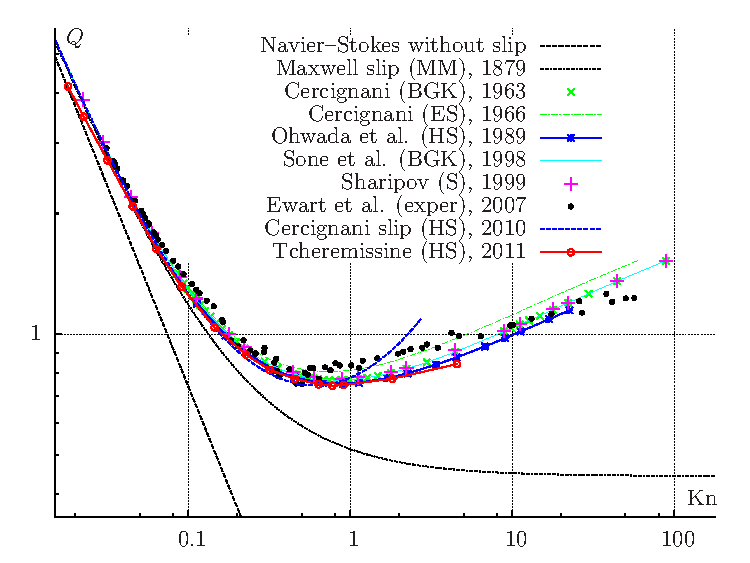
\includegraphics{problems/poiseuille.pdf}
	\caption{Зависимость потока массы \(Q\) от числа Кнудсена \(\Kn\).}\label{fig:graph}
\end{figure}

На рис.~\ref{fig:graph} представлены результаты решения задачи Пуазёйля описанными ранее методами.
Видно, что для линейной задачи модельные уравнения в общем дают близкие значения к истинным.
Экспериментальные данные также хорошо ложатся на теоретическую кривую,
несмотря на описанные выше приближения (модель твёрдых сфер с полным диффузным отражением).
Что касается значений, полученных проекционным методом при решении двумерной задачи,
то они в переходном режиме достаточно плотно прилегают к результатам численного решения Оувады и др.~\cite{Ohwada1989b},
на основании чего можно заключить о высокой точности проекционного метода.

Для малых чисел Кнудсена отклонение кривой объясняется неточной аппроксимацией межмолекулярного потенциала
на грубой скоростной сетке (радиусом 10 узлов и 3.4 тепловых скоростей).
Для сильно разреженного газа также наблюдается заниженное значение потока по этой же причине,
однако посредством образования выделенных пространственных направлений потока газа.

Таким образом, наилучшие результаты при малых вычислительных затратах проекционный метод показывает для переходного режима.
Для слабо разреженного газа необходимо, во-первых, использовать большие кубатурные сетки Коробова из-за большого шага по времени,
кроме того кинетический подход подразумевает использование размера координатной ячейки не более длины свободного пробега,
посколько это характерный размер существенных изменений функции распределения.
Вычислительные трудности для сильно разреженного газа связаны в основном с необходимостью в мелкой скоростной сетке
и в достаточном отношении длины канала к его ширине.

\subsubsection{Резюме}

Проекционным метод показал хорошую сходимость для переходного режима в двумерной геометрии,
полученные результаты совпали как с экспериментальными данными, так решением данной задачи другими численными методами.
В двумерной геометрии наблюдается б\textit{о}льшие трудности при моделировании сильно разреженного газа
ввиду характерного для методов дискретных ординат так называемого \textit{эффекта луча}:
дискретность скоростной сетки обуславливает выделенные направления движения газа в физическом пространстве.
